\documentclass[11pt,a4paper]{article}
\usepackage[textwidth=37em,vmargin=30mm]{geometry}
\usepackage{calc,xunicode,amsmath,amssymb,paralist,enumitem,tabu,booktabs,datetime2,xeCJK,xeCJKfntef,listings}
\usepackage{tocloft,fancyhdr,tcolorbox,xcolor,graphicx,eso-pic}

\usepackage[hidelinks]{hyperref}
\hypersetup{
    colorlinks=false,
    pdfpagemode=FullScreen,
    pdftitle={Web Digest - 2023-01-08}
}

\setdefaultleftmargin{2em}{2em}{1em}{1em}{1em}{1em}

\usepackage{xeCJK,xeCJKfntef}
\newcommand{\myvphantom}[0]{\vphantom{QWERTYUIOPASDFGHJKLZXCVBNMqwertyuiopasdfghjklzxcvbnm1234567890ςρθδφγηξλζχψβμ\"A}}
\xeCJKsetup{PunctStyle=plain,RubberPunctSkip=false,CJKglue=\myvphantom\hskip 0pt plus 0.1em minus 0.05em,CJKecglue=\myvphantom\hskip 0.22em plus 200pt}
\XeTeXlinebreaklocale "zh"
\XeTeXlinebreakskip = 0pt


\setmainfont[Numbers=Lining]{Brygada 1918}
\setromanfont[Numbers=Lining]{Brygada 1918}
\setsansfont[Numbers=Lining]{IBM Plex Sans}
\setmonofont{JetBrains Mono NL}
\setCJKmainfont{Noto Serif CJK SC}
\setCJKromanfont{Noto Serif CJK SC}
\setCJKsansfont{Noto Sans CJK SC}
\setCJKmonofont{Noto Sans CJK SC}

\setlength{\parindent}{0pt}
\setlength{\parskip}{8pt}
\linespread{1.15}

\lstset{
	basicstyle=\ttfamily\footnotesize,
	numbersep=5pt,
	backgroundcolor=\color{black!5},
	showspaces=false,
	showstringspaces=false,
	showtabs=false,
	tabsize=2,
	captionpos=b,
	breaklines=true,
	breakatwhitespace=true,
	breakautoindent=true,
	linewidth=\textwidth
}






\newcommand{\coverpic}[2]{
    % argv: itemurl, authorname
    Cover photo by #2~~~~(\href{#1}{#1})
}
\newcommand{\makeheader}[0]{
    \begin{center}
        
        \rmfamily\scshape
        \fontsize{62pt}{70pt}\selectfont
        WEB\hfill DIGEST
        
        \vfill
        % \vskip 30pt
        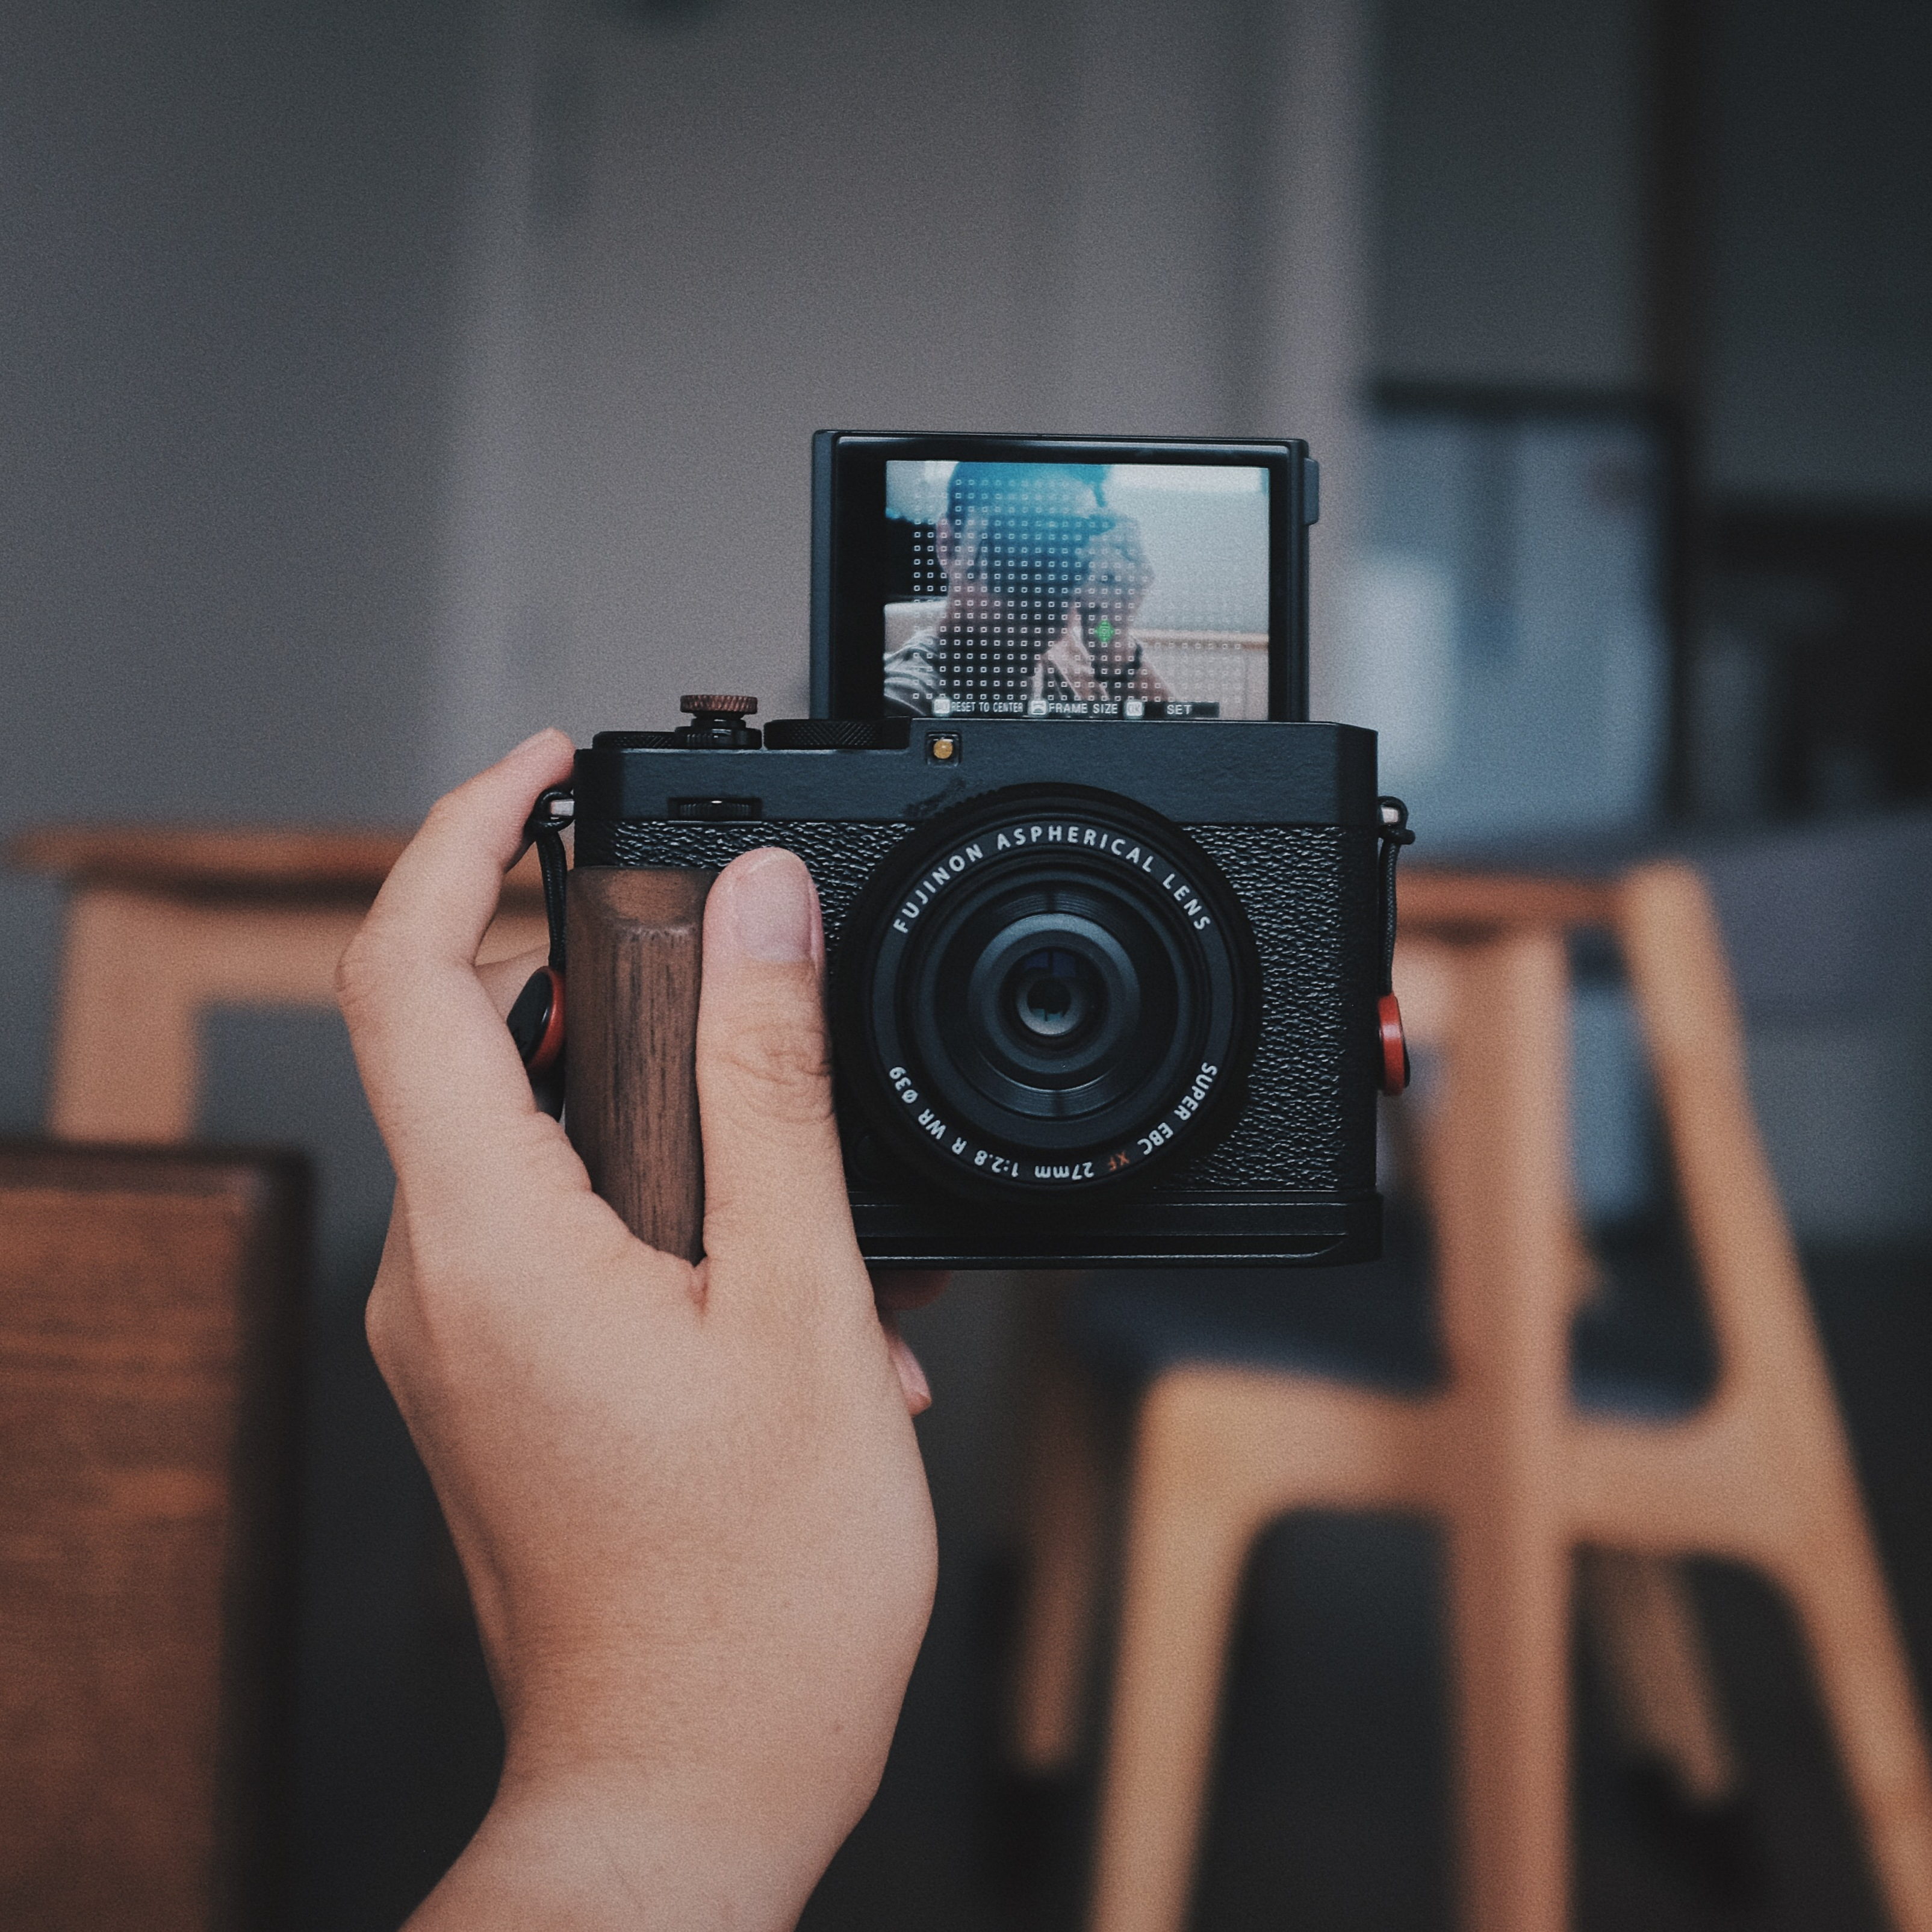
\includegraphics[width=\linewidth]{./today/coverpic.jpg}\par
        % \vskip 30pt
        \vfill

        \normalsize\upshape
        \copyright{} The Web Digest Project \hfill\large 2023-01-08
    \end{center}
    % \vskip 20pt
    % \hrule
    % \vskip 10pt
    % \clearpage
}
\renewcommand{\contentsname}{\center\Huge\sffamily\bfseries Contents\par\vskip 20pt}
\newcounter{ipartcounter}
\setcounter{ipartcounter}{0}
\newcommand{\ipart}[1]{
    % \vskip 20pt
    \clearpage
    \stepcounter{ipartcounter}
    \phantomsection
    \addcontentsline{toc}{section}{#1}
    \begin{center}
        \Huge
        \sffamily\bfseries
        #1
    \end{center}
    \vskip 20pt
}
\newcommand{\entrytitlefont}[0]{\Large\sffamily\bfseries}
\newcommand{\entryitemGeneric}[2]{
    % argv: title, url
    \parbox{\linewidth}{
        \entrytitlefont#1\par\vskip 5pt
        \footnotesize\ttfamily\mdseries
        \href{#2}{#2}\par
    }\vskip 11pt
}
\newcommand{\entryitemGithub}[3]{
    % argv: title, url, desc
    \parbox{\linewidth}{
        \entrytitlefont#1\par\vskip 5pt
        \footnotesize\ttfamily\mdseries
        \href{#2}{#2}\par\vskip 5pt
        \small\rmfamily\mdseries#3
    }\vskip 11pt
}
\newcommand{\entryitemAp}[3]{
    % argv: title, url, desc
    \parbox{\linewidth}{
        \entrytitlefont#1\par\vskip 5pt
        \footnotesize\ttfamily\mdseries
        \href{#2}{#2}\par\vskip 5pt
        \small\rmfamily\mdseries#3
    }\vskip 11pt
}
\newcommand{\entryitemHackernews}[3]{
    % argv: title, hnurl, rawurl
    \parbox{\linewidth}{
        \entrytitlefont#1\par\vskip 5pt
        \footnotesize\ttfamily\mdseries
        \href{#3}{#3}\par
        \textcolor{black!50}{\href{#2}{#2}}\par
    }\vskip 11pt
}






\begin{document}

\begin{titlepage}
	\makeheader
\end{titlepage}

\tableofcontents\clearpage


\ipart{Hacker News}
\entryitemHackernews{\hskip 0pt{}Will You Help Me Repair My Door [video]}{https://news.ycombinator.com/item?id=34293904}{https://www.youtube.com/watch?v=oponIfu5L3Y}

\entryitemHackernews{\hskip 0pt{}College that fired prof for showing image of Muhammad could lose accreditation}{https://news.ycombinator.com/item?id=34293131}{https://reason.com/2023/01/05/a-college-fired-a-professor-for-showing-a-painting-of-muhammad-now-it-could-lose-its-accreditation/}

\entryitemHackernews{\hskip 0pt{}The i3-gaps project has been merged with i3}{https://news.ycombinator.com/item?id=34293010}{https://github.com/Airblader/i3}

\entryitemHackernews{\hskip 0pt{}Jailbroken iOS can't run macOS apps – I spent a week to find out why (2021)}{https://news.ycombinator.com/item?id=34292795}{https://worthdoingbadly.com/macappsios/}

\entryitemHackernews{\hskip 0pt{}ChatGPT won't replace search engines any time soon}{https://news.ycombinator.com/item?id=34291565}{https://www.algolia.com/blog/ai/why-chatgpt-wont-replace-search-engines-any-time-soon/}

\entryitemHackernews{\hskip 0pt{}Production Twitter on one machine? 100Gbps NICs and NVMe are fast}{https://news.ycombinator.com/item?id=34291191}{https://thume.ca/2023/01/02/one-machine-twitter/}

\entryitemHackernews{\hskip 0pt{}Seattle Public Schools sues TikTok, YouTube, Instagram over youth mental health}{https://news.ycombinator.com/item?id=34291045}{https://www.geekwire.com/2023/seattle-public-schools-sues-tiktok-youtube-instagram-and-others-seeking-compensation-for-youth-mental-health-crisis/}

\entryitemHackernews{\hskip 0pt{}Excess management is costing the U.S. \$3T per year (2016)}{https://news.ycombinator.com/item?id=34290539}{https://hbr.org/2016/09/excess-management-is-costing-the-us-3-trillion-per-year}

\entryitemHackernews{\hskip 0pt{}Post-processing is ruining iPhone photos}{https://news.ycombinator.com/item?id=34290470}{https://9to5mac.com/2023/01/06/mkbhd-post-processing-ruining-iphone-photos/}

\entryitemHackernews{\hskip 0pt{}Microplastics are finding their way into fruit and vegetables as they grow}{https://news.ycombinator.com/item?id=34290129}{https://www.bbc.com/future/article/20230103-how-plastic-is-getting-into-our-food}

\entryitemHackernews{\hskip 0pt{}Show HN: Futurecoder – A free interactive Python course for coding beginners}{https://news.ycombinator.com/item?id=34289581}{https://futurecoder.io/}

\entryitemHackernews{\hskip 0pt{}The Safari bug that never was (2022)}{https://news.ycombinator.com/item?id=34289328}{https://obyford.com/posts/the-safari-bug-that-never-was/}

\entryitemHackernews{\hskip 0pt{}The Cornell Note Taking System}{https://news.ycombinator.com/item?id=34289310}{https://lsc.cornell.edu/how-to-study/taking-notes/cornell-note-taking-system/}

\entryitemHackernews{\hskip 0pt{}The science of having ideas in the shower}{https://news.ycombinator.com/item?id=34289138}{https://www.nationalgeographic.co.uk/history-and-civilisation/2022/08/the-science-of-why-you-have-great-ideas-in-the-shower}

\entryitemHackernews{\hskip 0pt{}Universal flu vaccine against all known subtypes takes promising first steps}{https://news.ycombinator.com/item?id=34289092}{https://www.science.org/doi/10.1126/science.abm0271}

\entryitemHackernews{\hskip 0pt{}Guitar Effects Guidebook, Vol. 20 [pdf]}{https://news.ycombinator.com/item?id=34288383}{https://static.roland.com/assets/media/pdf/guitar\_effects\_guidebook\_vol\_20.pdf}

\entryitemHackernews{\hskip 0pt{}Rsync.net warrant canary}{https://news.ycombinator.com/item?id=34287964}{https://www.rsync.net/resources/notices/canary.txt}

\entryitemHackernews{\hskip 0pt{}Study finds that buttons in cars are safer and quicker to use than touchscreens}{https://news.ycombinator.com/item?id=34287800}{https://futurism.com/the-byte/study-finds-that-buttons-in-cars-are-safer-and-quicker-to-use-than-touchscreens}

\entryitemHackernews{\hskip 0pt{}Ask HN: Main things to consider when building an app for business/enterprise?}{https://news.ycombinator.com/item?id=34287685}{https://news.ycombinator.com/item?id=34287685}

\entryitemHackernews{\hskip 0pt{}Not-such-better-living through chemistry}{https://news.ycombinator.com/item?id=34287564}{https://www.science.org/content/blog-post/not-such-better-living-through-chemistry}

\ipart{V2EX}
\entryitemGeneric{\hskip 0pt{}[分享发现] Juniper Junos 系统架构和命令模式浅谈}{https://www.v2ex.com/t/907332}

\entryitemGeneric{\hskip 0pt{}[程序员] Switch 有没有当做平板模式使用的配件}{https://www.v2ex.com/t/907330}

\entryitemGeneric{\hskip 0pt{}[奇思妙想] 有没有人做一个网页版微信,后台是固定在服务器上登陆的微信程序。}{https://www.v2ex.com/t/907329}

\entryitemGeneric{\hskip 0pt{}[问与答] 有没有阳完一直咳嗽的老哥去医院看过的,医生都给开了啥药啊?}{https://www.v2ex.com/t/907327}

\entryitemGeneric{\hskip 0pt{}[生活] 老婆下周生日,送点什么礼物好?}{https://www.v2ex.com/t/907326}

\entryitemGeneric{\hskip 0pt{}[问与答] QQ 被封号}{https://www.v2ex.com/t/907325}

\entryitemGeneric{\hskip 0pt{}[问与答] 如何调小 Win-10 , alt+tab 出来后的每个 app 预览窗口的大小?}{https://www.v2ex.com/t/907324}

\entryitemGeneric{\hskip 0pt{}[Safari] 无语的 bug #safari back-forward reload/refresh/back to the top}{https://www.v2ex.com/t/907321}

\entryitemGeneric{\hskip 0pt{}[分享发现] B 站搜索任何城市名 搜索结果被污染为垃圾视频}{https://www.v2ex.com/t/907319}

\entryitemGeneric{\hskip 0pt{}[问与答] 预算 2 万以下的一台做游戏的机器,目前看上了刃 9000k 或者 nuc 飞龙峡谷,哪个好呢}{https://www.v2ex.com/t/907318}

\entryitemGeneric{\hskip 0pt{}[Node.js] 测试马上删}{https://www.v2ex.com/t/907317}

\entryitemGeneric{\hskip 0pt{}[生活] 关于闲钱理财}{https://www.v2ex.com/t/907316}

\entryitemGeneric{\hskip 0pt{}[问与答] 有什么翻译工具或者翻译的 API 可以实现翻译文件里面的中文,保留英文?}{https://www.v2ex.com/t/907315}

\entryitemGeneric{\hskip 0pt{}[问与答] 请问有没有「比较经济的」「临时增加一台 mbp 或 studio 」的途径?}{https://www.v2ex.com/t/907314}

\entryitemGeneric{\hskip 0pt{}[问与答] 小白提问,如何让 Docker 容器不随着 SSH 客户端连接退出而结束}{https://www.v2ex.com/t/907313}

\entryitemGeneric{\hskip 0pt{}[问与答] skim 无法点击 pdf 里的超链接实现 pdf 内部的跳转吗?}{https://www.v2ex.com/t/907310}

\entryitemGeneric{\hskip 0pt{}[问与答] UHD 730 / 770 核显能带动 4K 屏幕吗}{https://www.v2ex.com/t/907309}

\entryitemGeneric{\hskip 0pt{}[C++] 谁 vscode remote SSL 遇到过循环刷 waiting for log 登不上去服务器的情况}{https://www.v2ex.com/t/907305}

\entryitemGeneric{\hskip 0pt{}[Apple] 關於帳戶地區和 IP 的問題}{https://www.v2ex.com/t/907304}

\entryitemGeneric{\hskip 0pt{}[剧集] 2022 年最喜欢的剧}{https://www.v2ex.com/t/907303}

\entryitemGeneric{\hskip 0pt{}[分享发现] 看到个有趣的背单词 app}{https://www.v2ex.com/t/907301}

\entryitemGeneric{\hskip 0pt{}[问与答] 12306 的订票排队,我这种情况还有可能买到票吗?}{https://www.v2ex.com/t/907300}

\entryitemGeneric{\hskip 0pt{}[Python] 基于 OpenAI 的 API, 实现上下文关联的 ChatGPT 对话工具}{https://www.v2ex.com/t/907298}

\entryitemGeneric{\hskip 0pt{}[分享发现] 本人经历诈骗惊险记---分享给各位提高警惕}{https://www.v2ex.com/t/907297}

\entryitemGeneric{\hskip 0pt{}[深圳] 求推荐深圳附近的度假村}{https://www.v2ex.com/t/907296}

\entryitemGeneric{\hskip 0pt{}[电影] 2022 年最喜欢的电影}{https://www.v2ex.com/t/907295}

\entryitemGeneric{\hskip 0pt{}[Chrome] mbp m2 13 寸, Chrome 几分钟后 cpu100\%就卡死}{https://www.v2ex.com/t/907294}

\entryitemGeneric{\hskip 0pt{}[分享发现] 我发现可以使用 OpenAI 来教自己一些基本的编程概念}{https://www.v2ex.com/t/907292}

\entryitemGeneric{\hskip 0pt{}[深圳] 深圳配隐形眼镜多少钱}{https://www.v2ex.com/t/907291}

\entryitemGeneric{\hskip 0pt{}[问与答] 吃素了一个月,发现性欲下降了}{https://www.v2ex.com/t/907290}

\entryitemGeneric{\hskip 0pt{}[macOS] mac 把文件从内置硬盘移动到移动硬盘,发现写入算内置硬盘?}{https://www.v2ex.com/t/907289}

\entryitemGeneric{\hskip 0pt{}[程序员] React Native 可以精简大小吗?在 Android 下默认就 55MB 了}{https://www.v2ex.com/t/907288}

\entryitemGeneric{\hskip 0pt{}[深圳] 有没有 14-15 号深圳回南阳的车, 2 个位。火车抢不到哇}{https://www.v2ex.com/t/907287}

\entryitemGeneric{\hskip 0pt{}[宽带症候群] 成都电信组播看 iptv}{https://www.v2ex.com/t/907285}

\entryitemGeneric{\hskip 0pt{}[分享创造] 开源 C 库实现 HTTP 服务器:多线程+事件模型+外挂式跟踪技术}{https://www.v2ex.com/t/907284}

\entryitemGeneric{\hskip 0pt{}[京东] 1.8 京东 PLUS 超级联名卡又开启耍猴模式}{https://www.v2ex.com/t/907280}

\entryitemGeneric{\hskip 0pt{}[问与答] 如何快速删除我所有的微信收藏?}{https://www.v2ex.com/t/907279}

\entryitemGeneric{\hskip 0pt{}[Java] 新手请教各位前辈 关于换项目和新技术的学习}{https://www.v2ex.com/t/907278}

\entryitemGeneric{\hskip 0pt{}[问与答] 微信支付的小微商户收款只能通过第三方来申请?}{https://www.v2ex.com/t/907277}

\entryitemGeneric{\hskip 0pt{}[前端开发] 使用 Taro 来构建一个小程序组件库,有什么可以抄作业的最佳实践吗?}{https://www.v2ex.com/t/907276}

\entryitemGeneric{\hskip 0pt{}[Apple] 现在 iPhone 无法关闭双重验证了吗}{https://www.v2ex.com/t/907275}

\entryitemGeneric{\hskip 0pt{}[分享发现] 各位城市最近行车状况如何,我感觉越临近过年,乱插的车越多}{https://www.v2ex.com/t/907274}

\entryitemGeneric{\hskip 0pt{}[分享发现] 《朗文当代高级英语词典》mac 版,适配原生 Dictionary APP}{https://www.v2ex.com/t/907272}

\entryitemGeneric{\hskip 0pt{}[macOS] 破案 Tab 键在 Safari 中刷题不是空格而是键盘巡航功能}{https://www.v2ex.com/t/907271}

\entryitemGeneric{\hskip 0pt{}[Windows] Microsoft store 老是出现``假更新''}{https://www.v2ex.com/t/907269}

\entryitemGeneric{\hskip 0pt{}[分享发现] 最近接触到 matrix 网桥,创建了一个通过 matrix 桥接 tg 和 discord 的联合群组,有兴趣的可以加入}{https://www.v2ex.com/t/907267}

\entryitemGeneric{\hskip 0pt{}[英雄联盟] 台服 LOL 也有 mac 版了}{https://www.v2ex.com/t/907266}

\entryitemGeneric{\hskip 0pt{}[程序员] 有接私活的吗 来一个}{https://www.v2ex.com/t/907265}

\entryitemGeneric{\hskip 0pt{}[程序员] PerimeterX 的按压验证 咋这么牛}{https://www.v2ex.com/t/907264}

\entryitemGeneric{\hskip 0pt{}[哔哩哔哩] 请教成功经验,怎么减少看 b 站?}{https://www.v2ex.com/t/907263}

\ipart{Solidot}
\entryitemGeneric{\hskip 0pt{}Debian 移除 Python 2}{https://www.solidot.org/story?sid=73791}

\entryitemGeneric{\hskip 0pt{}DistroWatch 的二十年}{https://www.solidot.org/story?sid=73790}

\entryitemGeneric{\hskip 0pt{}Linux Mint 21.1 释出}{https://www.solidot.org/story?sid=73717}

\entryitemGeneric{\hskip 0pt{}Linux 内核贡献成熟度模型}{https://www.solidot.org/story?sid=73677}

\entryitemGeneric{\hskip 0pt{}内核补丁将 kallsyms\_lookup\_name()查找速度提高 715 倍}{https://www.solidot.org/story?sid=73648}

\entryitemGeneric{\hskip 0pt{}Linux 6.1 释出}{https://www.solidot.org/story?sid=73621}

\entryitemGeneric{\hskip 0pt{}费米实验室和 CERN 选择 AlmaLinux}{https://www.solidot.org/story?sid=73595}

\entryitemGeneric{\hskip 0pt{}Steam Linux 市场份额达到 1.44\%}{https://www.solidot.org/story?sid=73543}

\entryitemGeneric{\hskip 0pt{}微软称 WSL 达到了 GA 阶段}{https://www.solidot.org/story?sid=73451}

\entryitemGeneric{\hskip 0pt{}Fedora 37 发布}{https://www.solidot.org/story?sid=73387}

\entryitemGeneric{\hskip 0pt{}开源 Linux 平板电脑,预装 FydeOS 出货}{https://www.solidot.org/story?sid=73256}

\entryitemGeneric{\hskip 0pt{}钓鱼网站在 Google 上伪装成 GIMP 打广告}{https://www.solidot.org/story?sid=73245}

\entryitemGeneric{\hskip 0pt{}Fedora Linux 37 为修复高危漏洞推迟发布}{https://www.solidot.org/story?sid=73198}

\entryitemGeneric{\hskip 0pt{}Rust for Linux 项目下一步发展计划}{https://www.solidot.org/story?sid=73165}

\entryitemGeneric{\hskip 0pt{}Linux 考虑淘汰对英特尔 i486 CPU 的支持}{https://www.solidot.org/story?sid=73155}

\entryitemGeneric{\hskip 0pt{}Ubuntu 22.10 Kinetic Kudu 发布}{https://www.solidot.org/story?sid=73140}

\entryitemGeneric{\hskip 0pt{}Tails 5.5 发布}{https://www.solidot.org/story?sid=73107}

\entryitemGeneric{\hskip 0pt{}Ubuntu 终端广告惹恼用户}{https://www.solidot.org/story?sid=73098}

\entryitemGeneric{\hskip 0pt{}Linus Torvalds 呼吁内核开发者不要在截止日期前递交补丁}{https://www.solidot.org/story?sid=73088}

\entryitemGeneric{\hskip 0pt{}Linux 6.1-rc1 释出}{https://www.solidot.org/story?sid=73081}

\ipart{联合早报}
\entryitemGeneric{\hskip 0pt{}召开全体会议前造势 中纪委通报高官落马播反腐专题片}{https://www.zaobao.com/news/china/story20230108-1351142}

\entryitemGeneric{\hskip 0pt{}春运启动 车站人头攒动}{https://www.zaobao.com/news/china/story20230108-1351143}

\entryitemGeneric{\hskip 0pt{}台湾拟10年内投入11亿元 进军国际太空产业}{https://www.zaobao.com/news/china/story20230108-1351144}

\entryitemGeneric{\hskip 0pt{}中国争取许可由国内制药商在华产销Paxlovid 研发首款mRNA疫苗进入试产}{https://www.zaobao.com/news/china/story20230108-1351145}

\entryitemGeneric{\hskip 0pt{}尽管大陆加大对台军事施压 美军舰通过台海次数去年降至四年新低}{https://www.zaobao.com/news/china/story20230108-1351146}

\entryitemGeneric{\hskip 0pt{}香港荣休主教陈日君 在梵蒂冈会见方济各}{https://www.zaobao.com/news/china/story20230108-1351147}

\entryitemGeneric{\hskip 0pt{}中国特斯拉降价 引发部分近期购车者抗议}{https://www.zaobao.com/news/china/story20230108-1351148}

\entryitemGeneric{\hskip 0pt{}官方研判同比增一倍 中国春运客流量今年料达近21亿人次}{https://www.zaobao.com/news/china/story20230107-1350822}

\entryitemGeneric{\hskip 0pt{}入境北京国际航班 下周四起直达不分流}{https://www.zaobao.com/news/china/story20230107-1350823}

\entryitemGeneric{\hskip 0pt{}美导弹驱逐舰穿越台海 中方称全程监视}{https://www.zaobao.com/news/china/story20230107-1350824}

\entryitemGeneric{\hskip 0pt{}中国与土库曼斯坦提升至全面战略伙伴关系}{https://www.zaobao.com/news/china/story20230107-1350825}

\entryitemGeneric{\hskip 0pt{}新闻人间: ``先声''胡福明离世}{https://www.zaobao.com/news/china/story20230107-1350826}

\entryitemGeneric{\hskip 0pt{}陆港明起三年来首通关 四口岸逾34万人预约}{https://www.zaobao.com/news/china/story20230107-1350827}

\entryitemGeneric{\hskip 0pt{}中石油与塔利班签合同 从阿富汗北部开采石油}{https://www.zaobao.com/news/china/story20230107-1350828}

\entryitemGeneric{\hskip 0pt{}庄慧良:还税``愚''民?}{https://www.zaobao.com/news/china/story20230107-1350829}

\entryitemGeneric{\hskip 0pt{}年货大街开市 台北年味渐浓}{https://www.zaobao.com/news/china/story20230107-1350830}

\entryitemGeneric{\hskip 0pt{}疑涉上千亿元深圳旧城改造计划 传恒大原执行总裁被警方带走调查}{https://www.zaobao.com/news/china/story20230107-1350831}

\entryitemGeneric{\hskip 0pt{}习近平小马可斯会谈 中菲重申维护地区稳定和平处理争议}{https://www.zaobao.com/news/china/story20230106-1350490}

\entryitemGeneric{\hskip 0pt{}封关近三年后1月8日起重开口岸 陆港恢复通关每天往返人数设限}{https://www.zaobao.com/news/china/story20230106-1350491}

\entryitemGeneric{\hskip 0pt{}担心陆港通关后疫情升温 香港民众蜂拥接种冠病疫苗}{https://www.zaobao.com/news/china/story20230106-1350492}

\entryitemGeneric{\hskip 0pt{}美台拟本月中旬 在台北举行贸易谈判}{https://www.zaobao.com/news/china/story20230106-1350493}

\entryitemGeneric{\hskip 0pt{}为疫情防控提供保障 李克强吁加强医疗物资调配}{https://www.zaobao.com/news/china/story20230106-1350494}

\entryitemGeneric{\hskip 0pt{}台七名军官涉大陆间谍案 四人被收押三人交保候传}{https://www.zaobao.com/news/china/story20230106-1350495}

\entryitemGeneric{\hskip 0pt{}早说}{https://www.zaobao.com/news/china/story20230106-1350496}

\ipart{AP News}
\entryitemAp{\hskip 0pt{}Jags return fumble for TD, beat Titans for AFC South title}{https://apnews.com/article/jacksonville-jaguars-los-angeles-chargers-sports-nfl-football-joshua-dobbs-245237965ff4389a7d33ce3e58732333}{Jacksonville Jaguars linebacker Josh Allen (41) returns a fumble for a touchdown as defensive end Arden Key (49) covers in the second half of an NFL football game against the Tennessee Titans, Saturday, Jan. 7, 2023, in }

\entryitemAp{\hskip 0pt{}Seattle schools sue tech giants over social media harm}{https://apnews.com/article/social-media-seattle-lawsuits-mental-health-965a8f373e3bfed8157571912cc3b542}{This combination of 2017-2022 photos shows the logos of Facebook, YouTube, TikTok and Snapchat on mobile devices. On Friday, Jan. 6, 2023, Seattle Public Schools filed a lawsuit in U.S. District Court, suing the tech...}

\entryitemAp{\hskip 0pt{}Travelers rush to take advantage of China reopening}{https://apnews.com/article/health-china-hong-kong-beijing-business-49e31dedb78fd24c1077b340ebdafa1f}{Workers wearing face masks walk by as travelers wait at the departure hall of the Lok Ma Chau station following the reopening of crossing border with mainland China, in Hong Kong, Sunday, Jan. 8, 2023. Travelers...}

\entryitemAp{\hskip 0pt{}Mahomes sets record, Chiefs beat Raiders for AFC's top seed}{https://apnews.com/article/kansas-city-chiefs-las-vegas-raiders-sports-nfl-football-damar-hamlin-5d08f366a1e2319104eb54ce22a570d2}{Kansas City Chiefs quarterback Patrick Mahomes runs with the ball against the Las Vegas Raiders during the first half of an NFL football game Saturday, Jan. 7, 2023, in Las Vegas. (AP Photo/John Locher) LAS VEGAS (AP) --}

\entryitemAp{\hskip 0pt{}On eve of Biden's border visit, migrants fear new rules}{https://apnews.com/article/biden-politics-el-paso-united-states-government-cuba-82701453fb018778c04255c1e2b10564}{A migrant, far left, reaches to bump fists with a local resident demonstrating in support of migrants in downtown El Paso, Texas, Saturday, Jan. 7, 2023. Several hundred marched through the streets of El Paso a day...}

\entryitemAp{\hskip 0pt{}Subway train collision in Mexico City kills 1, injures 57}{https://apnews.com/article/mexico-city-caribbean-accidents-5f604dfae19afaef940260065cd43e69}{A subway passenger, injured when two subway trains collided, is taken on a stretcher to a waiting ambulance, outside the Raza station in Mexico City, Saturday, Jan. 7, 2023. Authorities announced at least one person was }

\entryitemAp{\hskip 0pt{}Speaker McCarthy: A weakened leader or emboldened survivor?}{https://apnews.com/article/politics-united-states-house-of-representatives-kevin-mccarthy-government-e986c620149b72030bb418bd5fadb4a2}{House Speaker Kevin McCarthy of Calif., gestures towards the newly installed nameplate at his office after he was sworn in as speaker of the 118th Congress in Washington, early Saturday, Jan. 7, 2023. (AP Photo/ Matt...}

\entryitemAp{\hskip 0pt{}Golden Globes are back on TV, but are reform efforts enough?}{https://apnews.com/article/golden-globe-awards-hollywood-foreign-press-association-tv-television-9ee1a25e378b0c707dcd1f5f205c405b}{FILE - Event signage appears above the red carpet at the 77th annual Golden Globe Awards on Jan. 5, 2020, in Beverly Hills, Calif. The 80th annual Golden Globe Awards will take place on Tuesday, Jan. 10. (Photo by...}

\entryitemAp{\hskip 0pt{}Drugstores make slow headway on staffing problems}{https://apnews.com/article/health-business-medication-covid-pandemics-7aa39f8227449cc3b4e1bd2d3b130716}{Jessi Stout, owner of the Table Rock Pharmacy fills a prescription on Friday, Jan. 6, 2023, in Morganton, N.C. Drugstore chains are still trying to find enough employees to put a stop to temporary pharmacy closures. (AP }

\entryitemAp{\hskip 0pt{}Mayor: Teacher shot by 6-year-old 'red flag for the country'}{https://apnews.com/article/education-teaching-newport-news-virginia-38beb789647975e2f8f0d7c7447eb777}{Students and police gather outside of Richneck Elementary School after a shooting, Friday, Jan. 6, 2023 in Newport News, Va. A shooting at a Virginia elementary school sent a teacher to the hospital and ended with ``an...}

\entryitemAp{\hskip 0pt{}UK palace allies push back against Prince Harry's claims}{https://apnews.com/article/queen-elizabeth-ii-king-charles-iii-politics-united-kingdom-prince-harry-952c0cbaa0c39d18b8338ca651b49394}{This undated screengrab issued by ITV on Friday Jan. 6, 2023 shows Britain\textquotesingle s Prince Harry speaking during an interview with ITV\textquotesingle s Tom Bradby for the programme Harry: The Interview. (Harry:}

\entryitemAp{\hskip 0pt{}W.Va. journalist let go after reporting on abuse allegations}{https://apnews.com/article/west-virginia-state-government-jim-justice-af942f587d098b2d996cc6e01991d615}{This undated photo shows former West Virginia Public Broadcasting reporter Amelia Ferrell Knisely. Knisely was let go from her job at WVPB on Dec. 20, 2022, after she wrote about the alleged abuse of people with...}

\entryitemAp{\hskip 0pt{}A first for reclaimed Kyiv cathedral: Christmas in Ukrainian}{https://apnews.com/article/russia-ukraine-war-moscow-religion-orthodox-church-9bea8791e5eda36a0b01cb3b6da86bd5}{Metropolitan Epiphanius, center right, and priests deliver an Orthodox Christmas service inside the nearly 1,000-year-old Pechersk Lavra Cathedral of Kyiv, Ukraine, Saturday, Jan. 7, 2023. Hundreds of Ukrainians heard...}

\entryitemAp{\hskip 0pt{}Big week for US-Mexico ties going into North American summit}{https://apnews.com/article/biden-politics-mexico-government-us-national-security-council-united-states-599d640834d079503c5dd568c312c19f}{FILE - President Joe Biden speaks as he meets with Mexican President Andrés Manuel López Obrador in the Oval Office of the White House in Washington, July 12, 2022. Biden will become the first U.S. leader to visit...}

\entryitemAp{\hskip 0pt{}EXPLAINER: New drug slows Alzheimer's but comes with caveats}{https://apnews.com/article/health-medication-b42dc8b32d71f1b6892b07d85e0e7da0}{U.S. health officials have approved a new Alzheimer's drug that modestly slows the brain-robbing disease. (Jan. 6) This Dec. 21, 2022 image provided by Eisai in January 2023, shows vials and packaging for their...}

\entryitemAp{\hskip 0pt{}States target transgender health care in first bills of 2023}{https://apnews.com/article/politics-health-texas-state-government-tennessee-minnesota-878a9217fa434f3ecd83738a71e40572}{FILE - The Utah State Capitol is shown on Feb. 1, 2022, in Salt Lake City. After a midterm election and record flow of anti-transgender legislation in 2022, Republican state lawmakers this year are zeroing in on...}

\entryitemAp{\hskip 0pt{}Ukraine hails US military aid as cease-fire said to falter}{https://apnews.com/article/politics-united-states-government-ukraine-russia-war-moscow-9b3a132b330c90a10e8f031113be241b}{A cupola lies on the ground in front of the Orthodox Church which was destroyed by Russian forces in the recently retaken village of Bogorodychne, Ukraine, Saturday, Jan. 7, 2022. (AP Photo/Evgeniy Maloletka) KYIV...}

\entryitemAp{\hskip 0pt{}AP PHOTOS: Snow is a no-show as Europe feels the winter heat}{https://apnews.com/article/weather-climate-and-environment-droughts-europe-ac556a03360f361496aefb1c3a6569b6}{FILE - People ski on a cross country slope in Ramsau, Austria, Friday, Jan. 6, 2023. Sparse snowfall and unseasonably warm weather in much of Europe is allowing green grass to blanket many mountaintops across the region }

\entryitemAp{\hskip 0pt{}Chaos in the House: McCarthy's plea, and begging for votes}{https://apnews.com/article/politics-kevin-mccarthy-matt-gaetz-florida-f2a4a42b4845f2413cca5c1b4c6100dd}{Rep. Richard Hudson, R-N.C., left, pulls Rep. Mike Rogers, R-Ala., back as they talk with Rep. Matt Gaetz, R-Fla., and others during the 14th round of voting for speaker as the House meets for the fourth day to try and...}

\entryitemAp{\hskip 0pt{}Utah murder-suicide underscores frequency of family killings}{https://apnews.com/article/health-crime-utah-suicide-1e17fba2d7966f7436de96ddc974e530}{Jess, left, sits next to her sister, Cecily, during a press conference regarding the killing of a family in Enoch, Utah on Thursday, Jan. 5, 2023. A Utah man fatally shot his five children, his mother-in-law and his...}

\entryitemAp{\hskip 0pt{}Biden faces Israel quandary with new Netanyahu government}{https://apnews.com/article/biden-politics-israel-government-united-states-palestinian-territories-67a5be67c720bfa6c85d8d5a3050b65a}{FILE - Newly sworn-in Israeli Prime Minister Benjamin Netanyahu attends a cabinet meeting in Jerusalem, Dec. 29, 2022. Netanyahu\textquotesingle s new government is vexing the Biden administration as it embarks on...}

\entryitemAp{\hskip 0pt{}Mexican capo's arrest a gesture to US, not signal of change}{https://apnews.com/article/biden-mexico-andres-manuel-lopez-obrador-crime-medication-c4b7625503207540c2e821d8bf0e3ca6}{Army soldiers drive past a destroyed vehicle on the streets of Jesus Maria, Mexico, on Saturday, Jan. 7, 2023, the small town where Ovidio Guzman was detained earlier in the week. Thursday\textquotesingle s government...}

\entryitemAp{\hskip 0pt{}Heart screening may not have prevented Hamlin's collapse}{https://apnews.com/article/buffalo-bills-sports-health-heart-disease-youth-0c18b0c970a6af73fd9434a937517475}{FILE - Buffalo Bills\textquotesingle{} Damar Hamlin is examined during the first half of an NFL football game against the Cincinnati Bengals, Monday, Jan. 2, 2023, in Cincinnati. Quick on-the-field emergency care from...}

\entryitemAp{\hskip 0pt{}China suspends social media accounts of COVID policy critics}{https://apnews.com/article/health-china-government-covid-19-pandemic-beijing-3259cdf2fb41e8dd3d64f6c6d3b7cc80}{A man wearing a face mask shops for Chinese Lunar New Year decorations at a pavement store in Beijing, Saturday, Jan. 7, 2023. China has suspended or closed the social media accounts of more than 1,000 critics of the...}

\entryitemAp{\hskip 0pt{}Mega Millions jackpot rises to \$1.1 billion after no winner}{https://apnews.com/article/lotteries-business-91724709aa5fb0805e1bcf7157aad738}{Electrician Jose Valles, 59, from Rancho Cucamonga, Calif., buys a SuperLotto Plus ticket at the gas station that previously sold the \$2.04 billion-winning Powerball ticket award at Joe\textquotesingle s Service...}

\entryitemAp{\hskip 0pt{}Family of slain Utah family says husband took guns from home}{https://apnews.com/article/utah-divorce-suicide-b2742ac684ad5fb4b0b506efac85578b}{Jess, left, sits next to her sister, Cecily, during a press conference regarding the killing of a family in Enoch, Utah on Thursday, Jan. 5, 2023. A Utah man fatally shot his five children, his mother-in-law and his...}

\entryitemAp{\hskip 0pt{}CES 2023: Startups aim to reduce global food waste}{https://apnews.com/article/CES-2023-las-vegas-climate-technology-0d0e84044c3d5218b10dc032cd2ff3c4}{An exhibitor demonstrates the OneThird avocado ripeness checker during CES Unveiled before the start of the CES tech show, Tuesday, Jan. 3, 2023, in Las Vegas. More than a thousand startups are showcasing their products }

\entryitemAp{\hskip 0pt{}Old NASA satellite falling from sky this weekend, low threat}{https://apnews.com/article/science-oddities-aerospace-technology-national-aeronautics-and-space-administration-2b960095b8726632d53ebb103077007a}{In this photo made available by NASA, the space shuttle Challenger launches the Earth Radiation Budget Satellite in 1984. On Friday, Jan. 6, 2023, the U.S. space agency said the 38-year-old NASA satellite is about to...}

\entryitemAp{\hskip 0pt{}'RuPaul's Drag Race' cast push back against hate, threats}{https://apnews.com/article/rupaul-drag-race-threats-264b6f3ce1a161492226616ec6a9f201}{Drag performer Loosey LaDuca arrives at the season 15 premiere of "RuPaul's Drag Race" in New York on Thursday, Jan. 5, 2023. (AP Photo/John Carucci) Contestants from ``RuPaul's Drag Race'' talk new season at its...}

\entryitemAp{\hskip 0pt{}Bills uplifted by Hamlin's recovery, place focus on Patriots}{https://apnews.com/article/new-england-patriots-buffalo-bills-sports-nfl-football-damar-hamlin-10911df45ebe7be39dadb851f219dd67}{Crews clear snow from a parking lot near a sign showing support for Buffalo Bills safety Damar Hamlin outside Highmark Stadium on Wednesday, Jan. 4, 2023, in Orchard Park, N.Y. (AP Photo/Joshua Bessex) ORCHARD PARK, N.Y.}

\entryitemAp{\hskip 0pt{}EXPLAINER: How armored vehicles aid Ukraine at critical time}{https://apnews.com/article/politics-military-technology-ukraine-government-russia-war-2d59aae94a7ad8a5c22083e77d699417}{FILE - American soldiers drive a Bradley fighting vehicle during a joint exercise with Syrian Democratic Forces at the countryside of Deir Ezzor in northeastern Syria, Dec. 8, 2021. The U.S. and Germany are sending...}

\entryitemAp{\hskip 0pt{}NYC hospitals prep for nurse strike amid negotiations}{https://apnews.com/article/health-new-york-city-manhattan-business-covid-aa271a346234a352bba7abe67638b55b}{FILE - Zach Clapp, a nurse in the Pediatric Cardiac ICU at Mount Sinai Hospital signs a board demanding safe staffing during a rally by NYSNA nurses from NY Presbyterian and Mount Sinai, Tuesday, March 16, 2021, in New...}

\entryitemAp{\hskip 0pt{}Orthodox celebrate Christmas in shadow of conflict}{https://apnews.com/article/putin-ukraine-government-religion-e0d9f15655e18308c991997f7fc71cf7}{Russian Orthodox Patriarch Kirill delivers a Christmas service in the Christ the Saviour Cathedral in Moscow, Russia, Friday, Jan. 6, 2023. Orthodox Christians celebrate Christmas on Jan. 7, in accordance with the...}

\entryitemAp{\hskip 0pt{}Hawaii eruption not dangerous but offers spectacular sight}{https://apnews.com/article/volcanoes-kilauea-hawaii-climate-and-environment-0fd356cfa61a82c7977f88e428ae8200}{This photo provided by Janice Wei shows the eruption inside the summit crater of the Kilauea volcano on the Big Island of Hawaii, Thursday, Jan. 5, 2023. Hawaii\textquotesingle s Kilauea, one of the world\...}

\entryitemAp{\hskip 0pt{}Police: 6-year-old shoots teacher in Virginia classroom}{https://apnews.com/article/newport-news-virginia-88dfe91f65173cbbd198a8816a21b5be}{Police respond to a shooting at Richneck Elementary School, Friday, Jan. 6, 2023 in Newport News, Va. A shooting at a Virginia elementary school sent a teacher to the hospital and ended with ``an individual'' in custody }

\entryitemAp{\hskip 0pt{}Message from US asylum hopefuls: Financial sponsors needed}{https://apnews.com/article/biden-venezuela-mexico-spokane-violence-0eb316a474baed22f433359b0644320b}{Dr. Kyle Varner, second from the right, who sponsors and houses people through the Venezuelan humanitarian parole program, speaks at his house with program beneficiaries, from left, Maria Amare, Cesar Baez, Jenderson...}

\entryitemAp{\hskip 0pt{}EXPLAINER: What is ChatGPT and why are schools blocking it?}{https://apnews.com/article/what-is-chat-gpt-ac4967a4fb41fda31c4d27f015e32660}{A ChatGPT prompt is shown on a device near a public school in Brooklyn, New York, Thursday, Jan. 5, 2023. New York City school officials started blocking this week the impressive but controversial writing tool that can...}

\entryitemAp{\hskip 0pt{}US approves Alzheimer's drug that modestly slows disease}{https://apnews.com/article/health-medication-us-food-and-drug-administration-business-d2a155172735e00d2aa7baaeb8c24a9b}{This Dec. 21, 2022 image provided by Eisai in January 2023, shows vials and packaging for their medication Leqembi. On Friday, Jan. 6, 2023, U.S. health officials approved Leqembi, a new Alzheimer's drug that modestly...}

\entryitemAp{\hskip 0pt{}California gets brief lull after damaging 'bomb cyclone'}{https://apnews.com/article/weather-storms-california-climate-and-environment-b83bb05fa2d21796a85be9bfc690cf17}{Waves crash into a seawall in Pacifica, Calif., Friday, Jan. 6, 2023. California weather calmed Friday but the lull was expected to be brief as more Pacific storms lined up to blast into the state, where successive...}

\entryitemAp{\hskip 0pt{}WWE's Vince McMahon is back after misconduct investigation}{https://apnews.com/article/sports-vince-mcmahon-business-sexual-misconduct-d35dd1b3f197945181c0a3701f9939f5}{FILE - Vince McMahon stands at Republican state convention in Hartford, Conn., Friday, May 18, 2012. McMahon is rejoining the board of WWE several months after he stepped down as CEO and chairman of the sports...}

\entryitemAp{\hskip 0pt{}South Carolina US House district ruled racial gerrymander}{https://apnews.com/article/politics-south-carolina-state-government-hilton-head-island-charleston-9f48c6c7668b7b9404a7a9335d3a195a}{FILE - State Sen. Dick Harpootlian, D-Columbia, compares his proposed map of U.S. House districts drawn with 2020 U.S. Census data to a plan supported by Republicans on Thursday, Jan. 20, 2022, in Columbia, S.C. A panel }

\entryitemAp{\hskip 0pt{}Global food prices in 2022 hit record high amid drought, war}{https://apnews.com/article/russia-ukraine-inflation-health-business-climate-and-environment-00539505ec5db37de5877137b9febeb8}{FILE - Children stand near shelters at a camp for displaced people on the outskirts of Dollow, Somalia, Sept. 19, 2022. (AP Photo/Jerome Delay, File) ROME (AP) --- Global prices for food commodities like grain and...}

\entryitemAp{\hskip 0pt{}Bills' Hamlin breathing on his own, joins team via video}{https://apnews.com/article/bills-damar-hamlin-health-update-b1edba1849b580c3cd9ec2ea39a85d1e}{FILE - Buffalo Bills Damar Hamlin with his helmet off before playing the Los Angeles Rams during an NFL football game, Sept. 8, 2021, in Inglewood, Calif. The scenes of Hamlin\textquotesingle s on-field collapse after...}

\entryitemAp{\hskip 0pt{}Kremlin-ordered truce is uncertain amid mutual mistrust}{https://apnews.com/article/russia-ukraine-war-kremlin-ordered-truce-650d6c7930c80e61763a672d05757da8}{A local resident runs past a burning house hit by the Russian shelling in Kherson, Ukraine, on the Orthodox Christmas Eve Friday, Jan. 6, 2023. (AP Photo/LIBKOS) KYIV, Ukraine (AP) --- An uneasy quiet settled over Kyiv...}

\entryitemAp{\hskip 0pt{}Wall Street rallies on rate hopes, notches gain for the week}{https://apnews.com/article/inflation-business-united-states-government-federal-reserve-system-financial-markets-1192ebd20662f914bcc908c8b6d81c90}{The New York Stock Exchange is seen in New York, Thursday, Feb. 24, 2022. Markets are opening mostly higher on Wall Street Friday after a wild ride a day earlier. The S\&P 500 added 0.4\% in the early going, following...}

\entryitemAp{\hskip 0pt{}Best of CES 2023: Canine communication and a calming pillow}{https://apnews.com/article/ces2023-best-of-jan6-9d127822b54184e6c4d8313368667dc0}{Ducky demonstrates FluentPet dog communication buttons during the Pepcom Digital Experience before the start of the CES tech show, Wednesday, Jan. 4, 2023, in Las Vegas. (AP Photo/John Locher) LAS VEGAS (AP) --- Tech...}

\entryitemAp{\hskip 0pt{}Cooler hiring and milder pay gains could aid inflation fight}{https://apnews.com/article/us-jobs-report-jan6-2023-78943d9829087d93e9681426ca0c8ae2}{FILE - Construction workers work on a building in Philadelphia, Wednesday, Dec. 21, 2022. America's employers added a solid 223,000 jobs in December, evidence that the economy remains healthy yet also a sign that the...}

\entryitemAp{\hskip 0pt{}Mexico gives account of violence after 'Chapo' son nabbed}{https://apnews.com/article/politics-united-states-government-mexico-drug-crimes-city-d74ba460138c067ca538c862e3f0a5b0}{A police convoy patrols Culiacan, Sinaloa state, Mexico, Friday, Jan. 6, 2023. The government operation on Thursday to detain Ovidio Guzman, the son of imprisoned drug lord Joaquin ``El Chapo'' Guzman, unleashed...}

\entryitemAp{\hskip 0pt{}FTC proposes rule that would ban employee noncompete clauses}{https://apnews.com/article/biden-technology-politics-business-9fb699837e8bf8ecd9c70dcf27699dcf}{FILE - The Federal Trade Commission building in Washington is pictured on Jan. 28, 2015. The Federal Trade Commission is proposing a new rule that would prevent employers from imposing noncompete clauses on their...}

\entryitemAp{\hskip 0pt{}The Year of the Slap: Pop culture moments in 2022}{https://apnews.com/article/2022-major-pop-culture-moments-movies-music-fashion-6112da82e4b05559f3c67ce1970c15cf}{Taylor Swift was up. Elon Musk was in, out, in and maybe out again. Tom Cruise was back. BTS stepped aside, and so did Serena Williams, and Tom Brady too --- oops, scratch that. But the slap? The slap was everywhere...}

\ipart{GitHub}
\entryitemGithub{\hskip 0pt{}donnemartin/system-design-primer}{https://github.com/donnemartin/system-design-primer}{Learn how to design large-scale systems. Prep for the system design
interview. Includes Anki flashcards.\\
\strut \\
Language: Python\\
Stars: 207670\\
Forks: 37233}

\entryitemGithub{\hskip 0pt{}itwanger/toBeBetterJavaer}{https://github.com/itwanger/toBeBetterJavaer}{一份通俗易懂、风趣幽默的Java学习指南,内容涵盖Java基础、Java并发编程、Java虚拟机、Java企业级开发、Java面试等核心知识点。学Java,就认准Java
程序员进阶之路😄\\
\strut \\
Language: Java\\
Stars: 5592\\
Forks: 865}

\entryitemGithub{\hskip 0pt{}tw93/Pake}{https://github.com/tw93/Pake}{🤱🏻 Simply make any web page a desktop application using Rust. 🤱🏻
很简单的用 Rust 打包网页生成很小的桌面 App\\
\strut \\
Language: Rust\\
Stars: 7450\\
Forks: 456}

\entryitemGithub{\hskip 0pt{}AykutSarac/jsoncrack.com}{https://github.com/AykutSarac/jsoncrack.com}{🔮 Seamlessly visualize your JSON data instantly into graphs; paste,
import or fetch!\\
\strut \\
Language: TypeScript\\
Stars: 21219\\
Forks: 1060}

\entryitemGithub{\hskip 0pt{}rmcelreath/stat\_rethinking\_2023}{https://github.com/rmcelreath/stat\_rethinking\_2023}{Statistical Rethinking Course for Jan-Mar 2023\\
\strut \\
Language: Unknown\\
Stars: 795\\
Forks: 65}

\entryitemGithub{\hskip 0pt{}EddieHubCommunity/LinkFree}{https://github.com/EddieHubCommunity/LinkFree}{Connect to your audience with a single link. Showcase the content you
create and your projects in one place. Make it easier for people to
find, follow and subscribe.\\
\strut \\
Language: JavaScript\\
Stars: 1880\\
Forks: 1539}

\entryitemGithub{\hskip 0pt{}sindresorhus/awesome}{https://github.com/sindresorhus/awesome}{😎 Awesome lists about all kinds of interesting topics\\
\strut \\
Language: Unknown\\
Stars: 233269\\
Forks: 24719}

\entryitemGithub{\hskip 0pt{}jart/blink}{https://github.com/jart/blink}{tiniest x86-64-linux emulator\\
\strut \\
Language: C\\
Stars: 3459\\
Forks: 106}

\entryitemGithub{\hskip 0pt{}microsoft/Web-Dev-For-Beginners}{https://github.com/microsoft/Web-Dev-For-Beginners}{24 Lessons, 12 Weeks, Get Started as a Web Developer\\
\strut \\
Language: JavaScript\\
Stars: 62919\\
Forks: 9886}

\entryitemGithub{\hskip 0pt{}book-searcher-org/book-searcher}{https://github.com/book-searcher-org/book-searcher}{Create and search books index, create your private library.\\
\strut \\
Language: TypeScript\\
Stars: 4289\\
Forks: 288}

\entryitemGithub{\hskip 0pt{}AUTOMATIC1111/stable-diffusion-webui}{https://github.com/AUTOMATIC1111/stable-diffusion-webui}{Stable Diffusion web UI\\
\strut \\
Language: Python\\
Stars: 27716\\
Forks: 5171}

\ipart{Dribbble}
\entryitemGeneric{\hskip 0pt{}Portfolio design}{https://dribbble.com/shots/20300654}

\entryitemGeneric{\hskip 0pt{}Core Dashboard Builder - Customer Components}{https://dribbble.com/shots/20267926}

\entryitemGeneric{\hskip 0pt{}Transboard - mobile app}{https://dribbble.com/shots/20254390}

\entryitemGeneric{\hskip 0pt{}Illustration}{https://dribbble.com/shots/20281759}

\entryitemGeneric{\hskip 0pt{}2022}{https://dribbble.com/shots/20271837}

\entryitemGeneric{\hskip 0pt{}Socials — 3D Illustration}{https://dribbble.com/shots/20283657}

\entryitemGeneric{\hskip 0pt{}Moonbag - Creation Flow}{https://dribbble.com/shots/20300195}

\entryitemGeneric{\hskip 0pt{}Social analytics website interaction}{https://dribbble.com/shots/20284159}

\entryitemGeneric{\hskip 0pt{}Día de Muertos skull}{https://dribbble.com/shots/20291953}

\entryitemGeneric{\hskip 0pt{}Finance app interaction}{https://dribbble.com/shots/20274820}

\entryitemGeneric{\hskip 0pt{}Citrix Admin Dashboard: Analytics UX UI}{https://dribbble.com/shots/20203136}

\entryitemGeneric{\hskip 0pt{}2023}{https://dribbble.com/shots/20271197}

\entryitemGeneric{\hskip 0pt{}Quantively}{https://dribbble.com/shots/20302928}

\entryitemGeneric{\hskip 0pt{}Values Emblems}{https://dribbble.com/shots/20263897}

\entryitemGeneric{\hskip 0pt{}Logofolio - Update 2023}{https://dribbble.com/shots/20310365}

\entryitemGeneric{\hskip 0pt{}Home app product page}{https://dribbble.com/shots/20309020}

\entryitemGeneric{\hskip 0pt{}Collaborative Photo Editing Software UI}{https://dribbble.com/shots/20268513}

\entryitemGeneric{\hskip 0pt{}Illustration}{https://dribbble.com/shots/20302474}

\entryitemGeneric{\hskip 0pt{}Logo collection 2022}{https://dribbble.com/shots/20282455}

\entryitemGeneric{\hskip 0pt{}Camp Icons}{https://dribbble.com/shots/20273934}

\entryitemGeneric{\hskip 0pt{}Omnitype Branding}{https://dribbble.com/shots/20272431}

\entryitemGeneric{\hskip 0pt{}The Trailers: Concept Site Part 1}{https://dribbble.com/shots/20292416}

\entryitemGeneric{\hskip 0pt{}Flatfile Branding, brand assets, visual identity}{https://dribbble.com/shots/20203247}

\entryitemGeneric{\hskip 0pt{}Effy Branding}{https://dribbble.com/shots/20282218}





\clearpage
\leavevmode\vfill
\footnotesize

Copyright \copyright{} 2023-01-08 Neruthes and other contributors.

The entries listed in this newsletter may be copyrighted by their respective creators.

This newsletter is generated by the Web Digest project.

Newsletters are also delivered via Telegram channel\\
\CJKunderline{\href{https://t.me/webdigestchannel}{t.me/webdigestchannel}}.

This newsletter is available in PDF format at\\
\CJKunderline{\href{https://webdigest.pages.dev/}{webdigest.pages.dev}}.

The source code being used to generated this newsletter is available at\\
\CJKunderline{\href{https://github.com/neruthes/webdigest/}{github.com/neruthes/webdigest}}.


\coverpic{https://unsplash.com/photos/an-aerial-view-of-a-beach-with-trees-in-the-background-ciYs2jFPqJ4}{Aditya Chinchure}


\end{document}
